% The Diageo put, drawn: a study aid (not part of the submission)
% Waterfalls and flows of LVMH's "purchase commitments for minority interests' shares".
% Build: cd report/explainer && tectonic diageo-put-flows.tex
% Figures: data/processed/lvmh_nci_put.csv and report/notes/nci-put-diageo.md.
\documentclass[11pt,a4paper]{article}
\usepackage[a4paper,margin=2cm]{geometry}
\usepackage[T1]{fontenc}
\usepackage{sourceserifpro}
\usepackage[semibold]{sourcesanspro}
\renewcommand{\familydefault}{\sfdefault}
\usepackage{microtype}
\usepackage{xcolor}
\usepackage{tikz}
\usetikzlibrary{arrows.meta,positioning,calc,decorations.pathreplacing,patterns,patterns.meta}
\usepackage{pgfplots}
\pgfplotsset{compat=1.18}
\usepackage[hidelinks]{hyperref}

% ---- Palette: one meaning per colour, used the same way in every figure ------
\definecolor{brand}{HTML}{1B365D}   % the put liability (debt to Diageo)
\definecolor{lost}{HTML}{C4553A}    % goodwill plug / value written off against goodwill
\definecolor{book}{HTML}{8C939C}    % Diageo's share of MH book equity
\definecolor{gain}{HTML}{2F7D5B}    % profit or loss (IASB route)
\definecolor{ink}{HTML}{1E2329}
\definecolor{muted}{HTML}{5A5F66}
\definecolor{hair}{HTML}{C9CDD2}
\definecolor{paper}{HTML}{F4F1EA}

\color{ink}
\setlength{\parindent}{0pt}
\setlength{\parskip}{5pt}
\pagestyle{empty}

\newcommand{\kicker}[1]{{\footnotesize\bfseries\color{brand}\MakeUppercase{#1}}\par\vspace{1pt}}
\newcommand{\fighead}[2]{\vspace{6pt}\kicker{#1}{\large\bfseries #2\par}\vspace{2pt}}
\newcommand{\src}[1]{\par\vspace{2pt}{\scriptsize\color{muted}#1\par}}
\newcommand{\key}[2]{\tikz[baseline=-0.6ex]\fill[#1] (0,-0.09) rectangle (0.32,0.13);\,#2}

% Waterfall helpers (inside a pgfplots axis, numeric x)
\newcommand{\wbar}[4]{\fill[#4] (axis cs:#1-0.32,#2) rectangle (axis cs:#1+0.32,#3);}
\newcommand{\conn}[2]{\draw[muted!70, densely dashed, line width=0.4pt] (axis cs:#1+0.32,#2) -- (axis cs:#1+0.68,#2);}

\pgfplotsset{
  wf/.style={
    width=\linewidth, height=7.2cm, scale only axis=false,
    axis lines*=left, ymajorgrids, grid style={hair, line width=0.3pt},
    ymin=0, enlarge x limits=false,
    tick label style={font=\scriptsize, text=muted},
    xticklabel style={font=\scriptsize, text=ink, align=center, text width=1.75cm},
    ylabel style={font=\scriptsize, text=muted},
    /pgf/number format/1000 sep={,}, scaled ticks=false,
    major tick length=0pt, axis line style={hair},
    clip=false,
  },
}

\begin{document}

% ============================================================================
{\footnotesize\color{muted}LVMH \textperiodcentered{} IAS 32.23 \textperiodcentered{} note 1.13 and note 21 \textperiodcentered{} study aid}\par
\vspace{2pt}
{\huge\bfseries The Diageo put, drawn\par}
\vspace{4pt}
{\large Where the money sits, where it moves, and where it never shows up.\par}
\vspace{2pt}

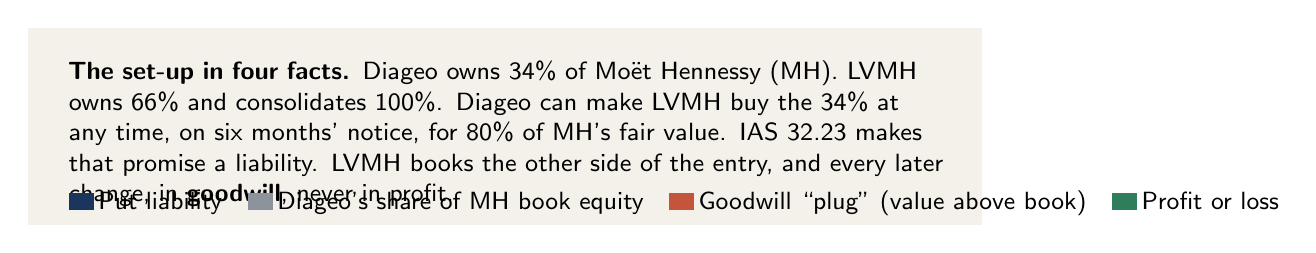
\begin{tikzpicture}
  \fill[paper] (0,0) rectangle (\linewidth,-2.5);
  \node[anchor=north west, text width=\linewidth-0.8cm, font=\small, align=left] at (0.4,-0.3) {%
    \textbf{The set-up in four facts.}
    Diageo owns 34\% of Mo\"et Hennessy (MH). LVMH owns 66\% and consolidates 100\%.
    Diageo can make LVMH buy the 34\% at any time, on six months' notice, for 80\% of MH's fair value.
    IAS~32.23 makes that promise a liability. LVMH books the other side of the entry, and every later change, in \textbf{goodwill}, never in profit.};
  \node[anchor=north west, font=\small] at (0.4,-1.95) {%
    \key{brand}{Put liability}\quad
    \key{book}{Diageo's share of MH book equity}\quad
    \key{lost}{Goodwill ``plug'' (value above book)}\quad
    \key{gain}{Profit or loss}};
\end{tikzpicture}

% ---------------------------------------------------------------------------
\fighead{1 \textperiodcentered{} The entry}{The liability is built from two blocks, and one of them has almost vanished}

Each year LVMH removes Diageo's minority interest from equity and writes up a put liability of 80\% of fair value. The gap between the two is parked in goodwill. Same scale for both years.

\begin{center}
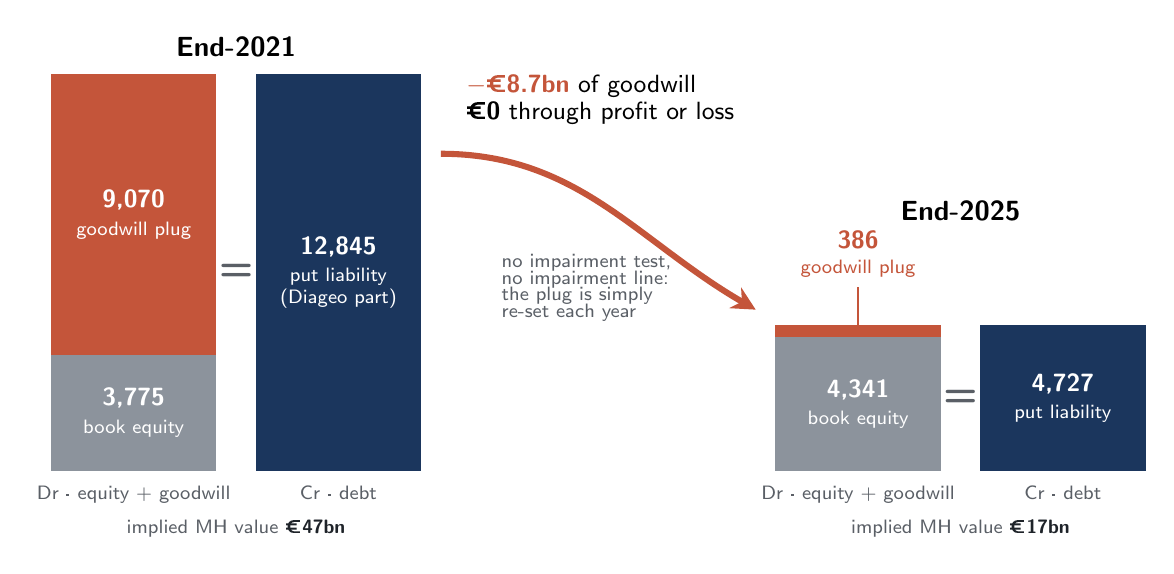
\begin{tikzpicture}[x=1cm, y=0.72cm, font=\small]
  % scale: 1 cm = EUR 1,835m  (12,845 -> 7.0 cm)
  \def\w{2.1}
  % ---------- 2021 ----------
  \begin{scope}[shift={(0,0)}]
    \fill[book] (0,0) rectangle (\w,2.057);
    \fill[lost] (0,2.057) rectangle (\w,7.000);
    \fill[brand] (\w+0.5,0) rectangle (2*\w+0.5,7.000);
    \node[white, align=center, font=\small\bfseries] at (\w/2,1.03) {3,775\\[-1pt]\scriptsize\mdseries book equity};
    \node[white, align=center, font=\small\bfseries] at (\w/2,4.53) {9,070\\[-1pt]\scriptsize\mdseries goodwill plug};
    \node[white, align=center, font=\small\bfseries] at (1.5*\w+0.5,3.5) {12,845\\[-1pt]\scriptsize\mdseries put liability\\[-3pt]\scriptsize\mdseries (Diageo part)};
    \node[font=\Large\bfseries, muted] at (\w+0.25,3.5) {=};
    \node[anchor=south, font=\normalsize\bfseries] at (\w+0.25,7.15) {End-2021};
    \node[anchor=north, font=\scriptsize, muted] at (\w/2,-0.08) {Dr \textperiodcentered{} equity + goodwill};
    \node[anchor=north, font=\scriptsize, muted] at (1.5*\w+0.5,-0.08) {Cr \textperiodcentered{} debt};
    \node[anchor=north, font=\scriptsize, muted] at (\w+0.25,-0.68) {implied MH value \textbf{\color{ink}\texteuro47bn}};
  \end{scope}
  % ---------- 2025 ----------
  \begin{scope}[shift={(9.2,0)}]
    \fill[book] (0,0) rectangle (\w,2.366);
    \fill[lost] (0,2.366) rectangle (\w,2.576);
    \fill[brand] (\w+0.5,0) rectangle (2*\w+0.5,2.576);
    \node[white, align=center, font=\small\bfseries] at (\w/2,1.18) {4,341\\[-1pt]\scriptsize\mdseries book equity};
    \draw[lost, line width=0.5pt] (\w/2,2.576) -- (\w/2,3.25) node[anchor=south, align=center, font=\small\bfseries, text=lost] {386\\[-2pt]\scriptsize\mdseries goodwill plug};
    \node[white, align=center, font=\small\bfseries] at (1.5*\w+0.5,1.29) {4,727\\[-1pt]\scriptsize\mdseries put liability};
    \node[font=\Large\bfseries, muted] at (\w+0.25,1.29) {=};
    \node[anchor=south, font=\normalsize\bfseries] at (\w+0.25,4.25) {End-2025};
    \node[anchor=north, font=\scriptsize, muted] at (\w/2,-0.08) {Dr \textperiodcentered{} equity + goodwill};
    \node[anchor=north, font=\scriptsize, muted] at (1.5*\w+0.5,-0.08) {Cr \textperiodcentered{} debt};
    \node[anchor=north, font=\scriptsize, muted] at (\w+0.25,-0.68) {implied MH value \textbf{\color{ink}\texteuro17bn}};
  \end{scope}
  % ---------- the bridge between them ----------
  \draw[-{Stealth[length=3mm,width=3mm]}, lost, line width=2.2pt] (4.95,5.6) to[out=0, in=150] (8.95,2.85);
  \node[align=left, font=\small, anchor=west] at (5.15,6.55) {\textbf{\color{lost}$-$\texteuro8.7bn} of goodwill\\[-1pt]\textbf{\texteuro0} through profit or loss};
  \node[align=left, font=\scriptsize, muted, anchor=north west] at (5.6,4.0) {no impairment test,\\[-2pt]no impairment line:\\[-2pt]the plug is simply\\[-2pt]re-set each year};
\end{tikzpicture}
\end{center}
\src{EUR m. Goodwill plug: FD 2021 note 4 (p.~41), FD 2025 note 4 (p.~40). Book equity: Diageo share of accumulated minority interests, FD 2021 note 17/18 (p.~52), FD 2025 note 18 (p.~53). Liability = sum of the two (the plug also holds small pre-2010 puts, so treat as ``about''). Implied MH value = liability $\div$ 0.8 $\div$ 0.34.}

% ---------------------------------------------------------------------------
\enlargethispage{3\baselineskip}
\fighead{2 \textperiodcentered{} The flow}{Follow FY2024: a \texteuro16bn fall in value, two possible exits}

\begin{center}
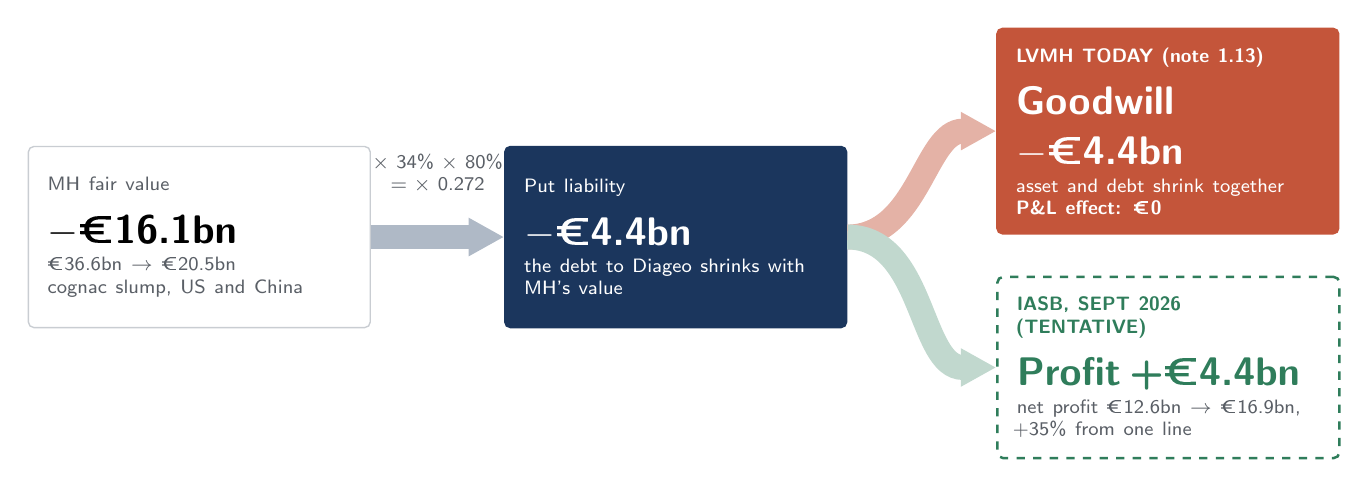
\begin{tikzpicture}[font=\small,
  card/.style={draw=hair, fill=white, line width=0.5pt, rounded corners=2pt, inner sep=7pt, align=left, text width=3.85cm, minimum height=2.3cm, anchor=north west, execute at begin node={\raggedright\hyphenpenalty=10000\exhyphenpenalty=10000}},
  band/.style={line width=9pt, -{Triangle[length=4.5mm,width=13pt]}},
]
  \node[card] (a) at (0,0) {{\scriptsize\color{muted}MH fair value\par}\vspace{1pt}{\Large\bfseries $-$\texteuro16.1bn\par}\vspace{2pt}{\scriptsize\color{muted}\texteuro36.6bn $\rightarrow$ \texteuro20.5bn\par cognac slump, US and China\par}};
  \node[card, fill=brand, draw=brand, text=white] (b) at (6.05,0) {{\scriptsize Put liability\par}\vspace{1pt}{\Large\bfseries $-$\texteuro4.4bn\par}\vspace{2pt}{\scriptsize the debt to Diageo shrinks with MH's value\par}};
  \draw[band, brand!35] (a.east) -- (b.west) node[midway, above=8pt, font=\scriptsize, text=muted, align=center] {$\times$ 34\% $\times$ 80\%\\$=\times$ 0.272};
  \node[card, fill=lost, draw=lost, text=white] (c1) at (12.3,1.5) {{\scriptsize\bfseries LVMH TODAY (note 1.13)\par}\vspace{1pt}{\Large\bfseries Goodwill $-$\texteuro4.4bn\par}\vspace{2pt}{\scriptsize asset and debt shrink together\par\textbf{P\&L effect: \texteuro0}\par}};
  \node[card, draw=gain, dashed, line width=0.9pt] (c2) at (12.3,-1.65) {{\scriptsize\bfseries\color{gain}IASB, SEPT 2026 (TENTATIVE)\par}\vspace{1pt}{\Large\bfseries\color{gain}Profit +\texteuro4.4bn\par}\vspace{2pt}{\scriptsize\color{muted}net profit \texteuro12.6bn $\rightarrow$ \texteuro16.9bn, +35\% from one line\par}};
  \draw[band, lost!45] (b.east) to[out=0, in=180] (c1.west);
  \draw[band, gain!30] (b.east) to[out=0, in=180] (c2.west);
\end{tikzpicture}
\end{center}

The counter-intuitive bit: when Diageo's stake loses value, LVMH owes Diageo less. Under the IASB route a \emph{collapse} shows up as a \emph{gain}; LVMH's route hides both. Rule of thumb: every \texteuro1bn of MH value moves the liability by about \texteuro0.27bn.
\src{FY2024. MH value: FD 2023/2024 notes 4, 18. Goodwill movement $-$\texteuro4,378m: FD 2024 note 4 (p.~40). Net profit: FD 2025 p.~24. IASB Update, Sept 2026. Pre-tax.}

\newpage
% ---------------------------------------------------------------------------
\fighead{3 \textperiodcentered{} The bridge}{From \texteuro13.7bn to \texteuro6.3bn: almost all of it is lost value, booked against goodwill}

The balance-sheet line ``purchase commitments for minority interests' shares'', end-2021 to end-2025. Each orange step is one year's fall in the goodwill plug, i.e. one year's fall in what LVMH thinks MH is worth above book.

\begin{center}
\begin{tikzpicture}
\begin{axis}[wf,
  xmin=0.45, xmax=8.55, ymax=16000,
  ytick={0,4000,8000,12000,16000},
  ylabel={EUR m},
  xtick={1,...,8},
  xticklabels={
    {\textbf{Liability}\\end-2021\\[-1pt]\color{muted}MH \texteuro47bn},
    {2022\\\color{muted}MH \texteuro41bn},
    {2023\\\color{muted}MH \texteuro37bn},
    {2024\\\color{muted}MH \texteuro20bn},
    {2025\\\color{muted}MH \texteuro17bn},
    {Diageo's book equity grows},
    {Other puts, net},
    {\textbf{Liability}\\end-2025}},
]
  \addplot[draw=none, forget plot] coordinates {(1,0)};
  % totals and steps (EUR m)
  \wbar{1}{0}{13677}{brand}
  \wbar{2}{11506}{13677}{lost}
  \wbar{3}{10289}{11506}{lost}
  \wbar{4}{5846}{10289}{lost}
  \wbar{5}{4993}{5846}{lost}
  \wbar{6}{4993}{5559}{book}
  \wbar{7}{5559}{6331}{book!55}
  \wbar{8}{0}{6331}{brand}
  % connectors
  \conn{1}{13677} \conn{2}{11506} \conn{3}{10289} \conn{4}{5846}
  \conn{5}{4993} \conn{6}{5559} \conn{7}{6331}
  % value labels
  \node[anchor=south, font=\small\bfseries] at (axis cs:1,13677) {13,677};
  \node[anchor=north, font=\scriptsize\bfseries, text=lost] at (axis cs:2,11506) {$-$2,171};
  \node[anchor=north, font=\scriptsize\bfseries, text=lost] at (axis cs:3,10289) {$-$1,217};
  \node[anchor=north, font=\scriptsize\bfseries, text=lost] at (axis cs:4,5846) {$-$4,443};
  \node[anchor=north, font=\scriptsize\bfseries, text=lost] at (axis cs:5,4993) {$-$853};
  \node[anchor=south, font=\scriptsize\bfseries, text=muted] at (axis cs:6,5559) {+566};
  \node[anchor=south, font=\scriptsize\bfseries, text=muted] at (axis cs:7,6331) {+772};
  \node[anchor=south, font=\small\bfseries] at (axis cs:8,6331) {6,331};
  % brace over the goodwill steps
  \draw[decorate, decoration={brace, amplitude=6pt}, line width=0.6pt, lost]
    (axis cs:1.62,14250) -- (axis cs:5.38,14250);
  \node[anchor=south, align=center, font=\small, text=ink] at (axis cs:3.5,14650)
    {\textbf{\color{lost}$-$\texteuro8.7bn} against goodwill \textperiodcentered{} \textbf{\texteuro0} through profit or loss};
  % callout on the 2024 step
  \draw[muted, line width=0.4pt] (axis cs:4.34,8100) -- (axis cs:4.75,8900)
    node[anchor=south west, align=left, font=\scriptsize, text=muted, inner sep=1pt]
    {2024 alone: W\&S intangibles\\[-2pt]and goodwill fell \texteuro5.4bn\\[-2pt]with no impairment charge};
\end{axis}
\end{tikzpicture}
\end{center}
\src{EUR m. Liability: FD 2021 and FD 2025 balance sheets (p.~26). Goodwill steps = change in ``goodwill arising on purchase commitments'' balance, FD 2021--25 note 4 (sum $-$8,684; the note-4 movement line sums to $-$8,717, the gap is FX and other). Book equity: note 18. Other puts, net = residual (Loro Piana, Middle-East distributors; post-2010 puts that go through equity). W\&S intangibles: FD 2025 note 24.1 (pp.~62--63).}

% ---------------------------------------------------------------------------
\fighead{4 \textperiodcentered{} The cash}{Money out to Diageo: a trickle every year, a wave on six months' notice}

\begin{center}
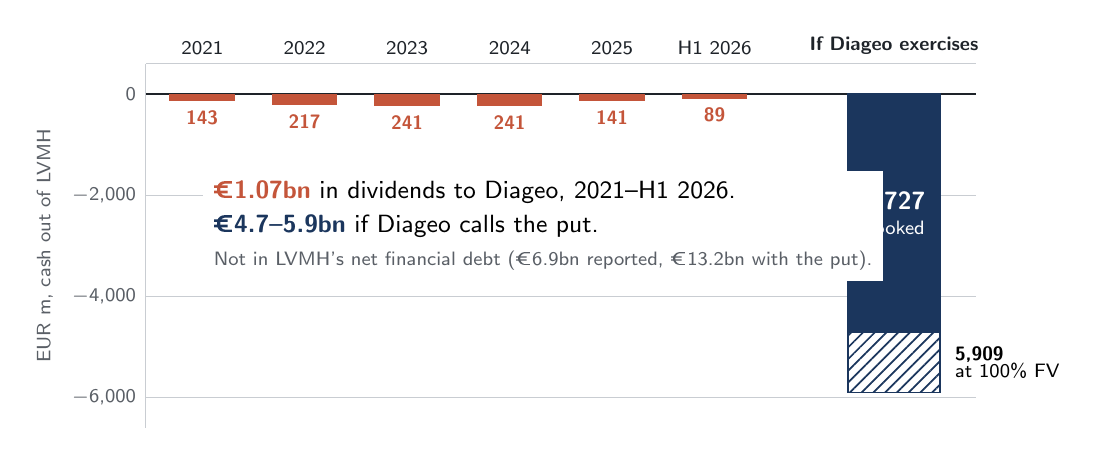
\begin{tikzpicture}
\begin{axis}[wf, height=6.2cm,
  xmin=0.45, xmax=8.55, ymin=-6600, ymax=600,
  ytick={-6000,-4000,-2000,0},
  yticklabels={{$-$6,000},{$-$4,000},{$-$2,000},0},
  ylabel={EUR m, cash out of LVMH},
  xtick={1,...,6,7.75},
  xticklabels={2021,2022,2023,2024,2025,H1 2026,{\textbf{If Diageo exercises}}},
  xticklabel style={text width=2.6cm},
  xticklabel pos=upper, axis x line*=top,
]
  \addplot[draw=none, forget plot] coordinates {(1,0)};
  \draw[ink, line width=0.6pt] (axis cs:0.45,0) -- (axis cs:8.55,0);
  \wbar{1}{-143}{0}{lost}
  \wbar{2}{-217}{0}{lost}
  \wbar{3}{-241}{0}{lost}
  \wbar{4}{-241}{0}{lost}
  \wbar{5}{-141}{0}{lost}
  \wbar{6}{-89}{0}{lost}
  \foreach \x/\v/\t in {1/143/143, 2/217/217, 3/241/241, 4/241/241, 5/141/141, 6/89/89}
    {\edef\tmp{\noexpand\node[anchor=north, font=\noexpand\scriptsize\noexpand\bfseries, text=lost] at (axis cs:\x,-\v) {\t};}\tmp}
  % exercise bar
  \fill[brand] (axis cs:7.3,-4727) rectangle (axis cs:8.2,0);
  \fill[pattern={Lines[angle=45, distance=3pt, line width=0.6pt]}, pattern color=brand]
    (axis cs:7.3,-5909) rectangle (axis cs:8.2,-4727);
  \draw[brand, line width=0.6pt] (axis cs:7.3,-5909) rectangle (axis cs:8.2,0);
  \node[white, font=\small\bfseries, align=center] at (axis cs:7.75,-2360) {4,727\\[-2pt]\scriptsize\mdseries booked};
  \node[anchor=west, font=\scriptsize, align=left] at (axis cs:8.25,-5318) {\textbf{5,909}\\[-2pt]at 100\% FV};
  % summary
  \node[anchor=north west, align=left, font=\small, fill=white, inner sep=4pt] at (axis cs:1.0,-1500)
    {\textbf{\color{lost}\texteuro1.07bn} in dividends to Diageo, 2021--H1 2026.\\[1pt]
     \textbf{\color{brand}\texteuro4.7--5.9bn} if Diageo calls the put.\\[1pt]
     \color{muted}\scriptsize Not in LVMH's net financial debt (\texteuro6.9bn reported, \texteuro13.2bn with the put).};
\end{axis}
\end{tikzpicture}
\end{center}
\src{Dividends paid to Diageo: FD 2021--25 note 17/18 (pp.~52--53); H1-2026 HFR note 18 (p.~42). Exercise: FD 2025 note 21 (p.~56), six months' notice at 80\% of fair value. Net financial debt excludes purchase commitments: FD 2025 note 19.1 (p.~53).}

\newpage
% ---------------------------------------------------------------------------
\fighead{5 \textperiodcentered{} The price}{What the acquirer would really pay for Diageo's 34\%}

The balance sheet shows one number. It is 80\% of a DCF taken at the bottom of the cognac cycle. The ladder below climbs from the partner's own valuation to the pre-slump one.

\begin{center}
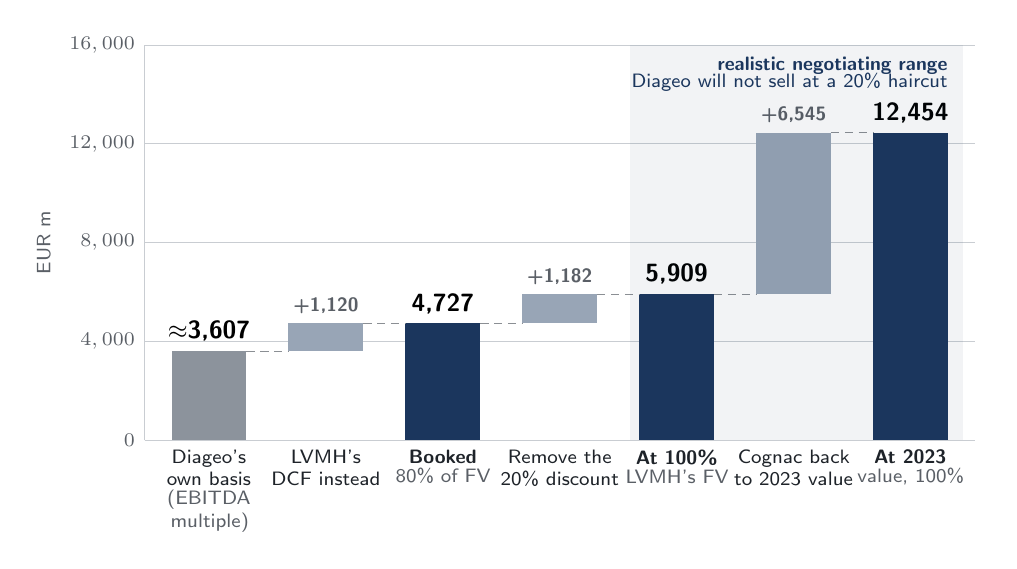
\begin{tikzpicture}
\begin{axis}[wf, height=6.6cm,
  xmin=0.45, xmax=7.55, ymax=16000,
  ytick={0,4000,8000,12000,16000},
  ylabel={EUR m},
  xtick={1,...,7},
  xticklabels={
    {Diageo's own basis\\[-1pt]\color{muted}(EBITDA multiple)},
    {LVMH's DCF instead},
    {\textbf{Booked}\\[-1pt]\color{muted}80\% of FV},
    {Remove the 20\% discount},
    {\textbf{At 100\%}\\[-1pt]\color{muted}LVMH's FV},
    {Cognac back to 2023 value},
    {\textbf{At 2023}\\[-1pt]\color{muted}value, 100\%}},
]
  \addplot[draw=none, forget plot] coordinates {(1,0)};
  \wbar{1}{0}{3607}{book}
  \wbar{2}{3607}{4727}{brand!45}
  \wbar{3}{0}{4727}{brand}
  \wbar{4}{4727}{5909}{brand!45}
  \wbar{5}{0}{5909}{brand}
  \wbar{6}{5909}{12454}{brand!45}
  \wbar{7}{0}{12454}{brand}
  \conn{1}{3607} \conn{2}{4727} \conn{3}{4727} \conn{4}{5909} \conn{5}{5909} \conn{6}{12454}
  \node[anchor=south, font=\small\bfseries] at (axis cs:1,3607) {$\approx$3,607};
  \node[anchor=south, font=\scriptsize\bfseries, text=muted] at (axis cs:2,4727) {+1,120};
  \node[anchor=south, font=\small\bfseries] at (axis cs:3,4727) {4,727};
  \node[anchor=south, font=\scriptsize\bfseries, text=muted] at (axis cs:4,5909) {+1,182};
  \node[anchor=south, font=\small\bfseries] at (axis cs:5,5909) {5,909};
  \node[anchor=south, font=\scriptsize\bfseries, text=muted] at (axis cs:6,12454) {+6,545};
  \node[anchor=south, font=\small\bfseries] at (axis cs:7,12454) {12,454};
  % shaded realistic band
  \fill[brand, opacity=0.06] (axis cs:4.6,0) rectangle (axis cs:7.45,16000);
  \node[anchor=north east, align=right, font=\scriptsize, text=brand] at (axis cs:7.4,15900)
    {\textbf{realistic negotiating range}\\[-2pt]Diageo will not sell at a 20\% haircut};
\end{axis}
\end{tikzpicture}
\end{center}
\src{EUR m, Diageo's part only. Booked = goodwill plug + book equity, FD 2025 notes 4 and 18 (pp.~40, 53). 100\% = 4,727 $\div$ 0.8. 2023 value = 9,963 $\div$ 0.8 (FD 2023 notes 4 and 18). Diageo's basis: solved from Diageo AR 2026 note 6 (printed p.~157) impairment sensitivity; different date, FX and policies, so indicative only.}

\end{document}
